\documentclass[10pt,xcolor=pdflatex,dvipsnames,table]{beamer}
\usepackage{newcent}
\usepackage[utf8]{inputenc}
\usepackage[czech]{babel}
\usepackage{hyperref}
\usepackage{amsthm}
\usepackage{amssymb}
\usepackage{amsmath}
\usepackage{array}
\usepackage{stmaryrd}
\usepackage{graphicx}
\usepackage{tabularx}
\usepackage{listings}
\usepackage{fancyvrb}
\usepackage{minted}
%\usepackage{packages/beamerthemeFIT}

\makeatletter
  \def\beamer@calltheme#1#2#3{%
    \def\beamer@themelist{#2}
    \@for\beamer@themename:=\beamer@themelist\do
    {\usepackage[{#1}]{\beamer@themelocation/#3\beamer@themename}}}

  \def\usefolder#1{
    \def\beamer@themelocation{#1}
  }
  \def\beamer@themelocation{}

\usefolder{packages}
\usetheme{FIT}

\title[CMake]{CMake Tutoriál}

\author[]{Tomáš Milet}

\institute[]{Brno University of Technology, Faculty of Information Technology\\
Bo\v{z}et\v{e}chova 1/2. 612 66 Brno - Kr\'alovo Pole\\
imilet@fit.vutbr.cz}

\date{\today}

\begin{document}

\frame[plain]{\titlepage}

\setbeamercolor{background canvas}{bg=fitblue}
\begin{frame}
\frametitle{Úvod}
\begin{center}
\Huge {\color{white}Úvod}
\end{center}
\end{frame}
\setbeamercolor{background canvas}{bg=white}

\begin{frame}
\frametitle{Zdroje informací}
	\begin{itemize}
  \item \url{https://cmake.org/cmake/help/v3.13/}
  \item \url{https://www.youtube.com/watch?v=bsXLMQ6WgIk}
  \item \url{https://pabloariasal.github.io/2018/02/19/its-time-to-do-cmake-right/}
	\end{itemize}
\end{frame}

\begin{frame}
\frametitle{Proč použít?}
	\begin{itemize}
	\item Multiplatformní
  \item Usnadňuje práci (závislosti, nastavení, ...)
  \item Standardizuje sestavování
  \item Testy, balíčky, uživatelské skripty, ...
  \item Out of source building, ...
	\end{itemize}
	\begin{figure}[h]
	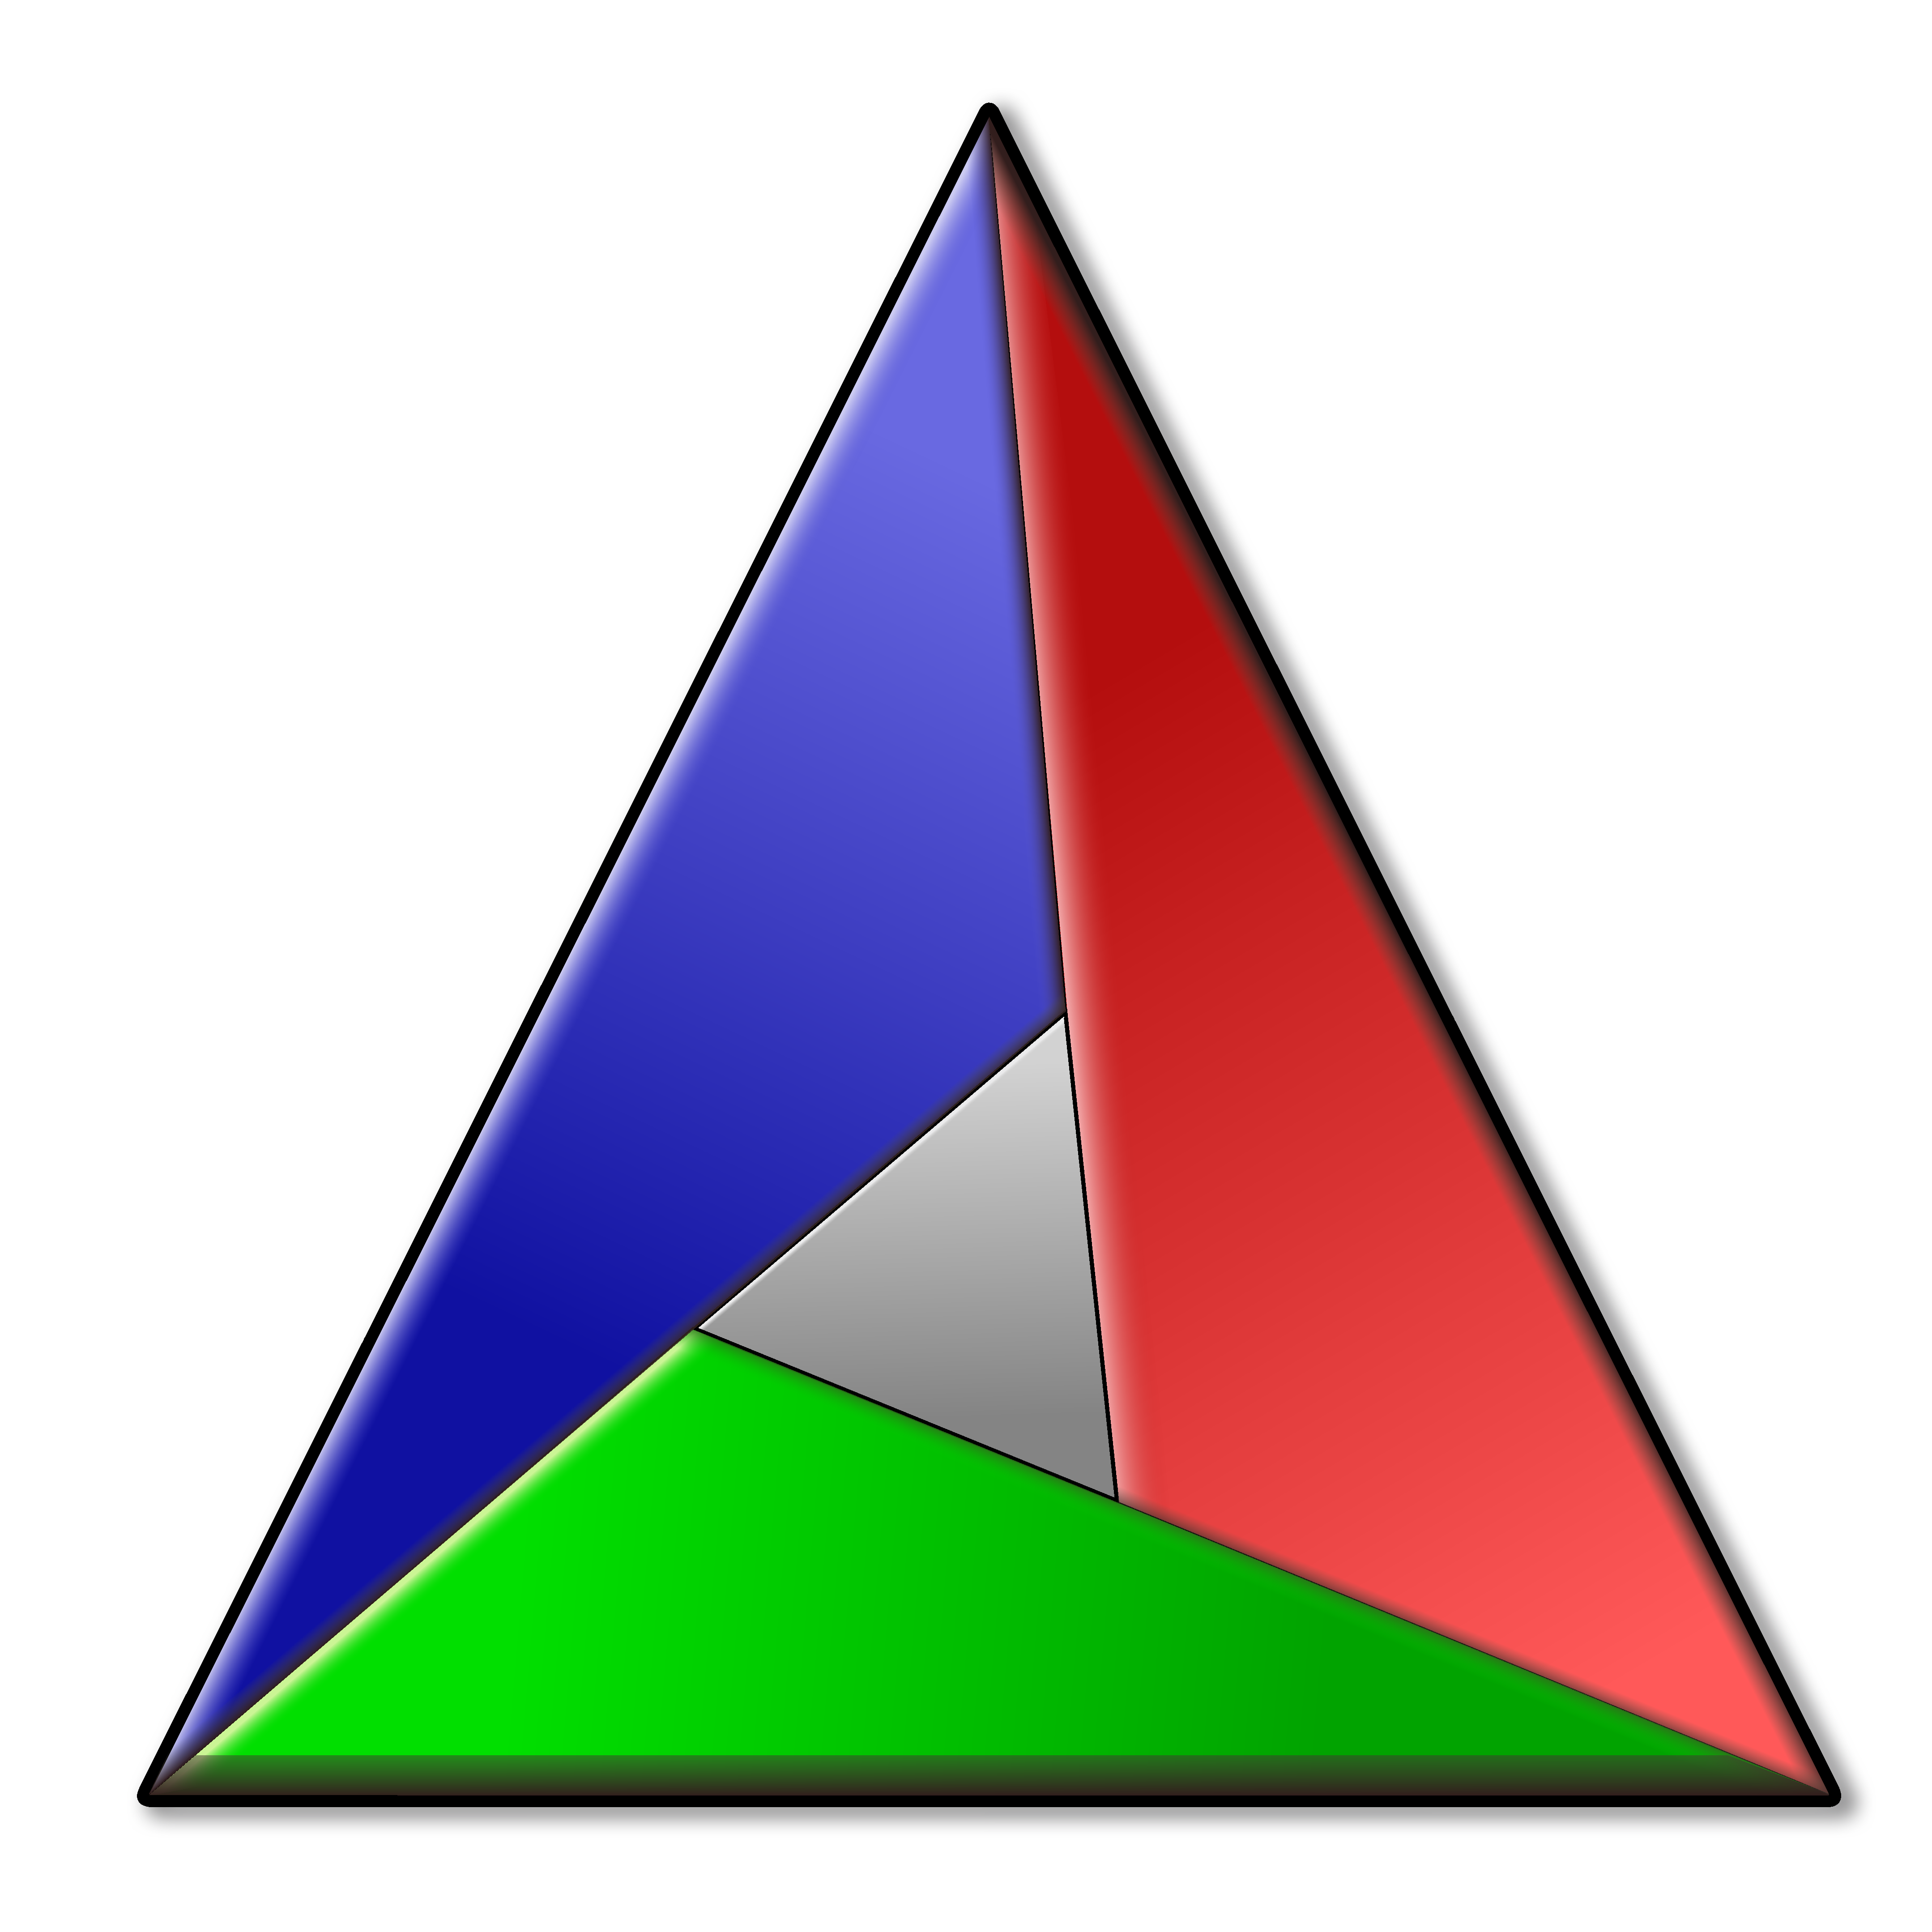
\includegraphics[width=2cm,keepaspectratio]{pics/introduction/Cmake}
	
\includegraphics[width=2cm,keepaspectratio]{pics/introduction/Tux}
	
\includegraphics[width=2cm,keepaspectratio]{pics/introduction/Windows}
	
\includegraphics[width=2cm,keepaspectratio]{pics/introduction/Apple}
	\end{figure}
\end{frame}

\begin{frame}[fragile]
\frametitle{Jak nainstalovat pod Linuxem?}
	\begin{enumerate}
    \item Odinstalovat všechny starší verze (najít třeba pomocí \$ \textbf{which} cmake)
    \item Stáhnout nejnovější binárni tar.gr verzi z \url{https://cmake.org/download/}
    \item Překopírovat obsah rozbaleného adresáře do /usr
	\end{enumerate}
{\scriptsize
\begin{Verbatim}[commandchars=\\\{\}]
$ \textbf{wget} https://cmake.org/files/v3.13/cmake-3.13.0-rc1-Linux-x86_64.tar.gz
$ \textbf{tar} xf cmake-3.13.0-rc1-Linux-x86_64.tar.gz
$ \textbf{cd} cmake-3.13.0-rc1-Linux-x86_64
$ \textbf{sudo cp} -r * /usr
$ \textbf{cmake} --version
cmake version 3.13.0-rc1
\end{Verbatim}
}
\end{frame}

\begin{frame}
\frametitle{Jak použít?}
{\scriptsize
	\begin{enumerate}
	\item cmake-gui / ccmake
	\item Nastavit místo, kde se sestavuje a kde je složka s CMakeLists.txt
	\item Configure
	\item Vyřešit závislosti - například nastavit SDL2\_DIR na složku obsahující SDL2Config.cmake
  \item Generate - vygenerovat makefile / sln file
  \item make / pustit MSVS
	\end{enumerate}
}
	\begin{figure}[h]
	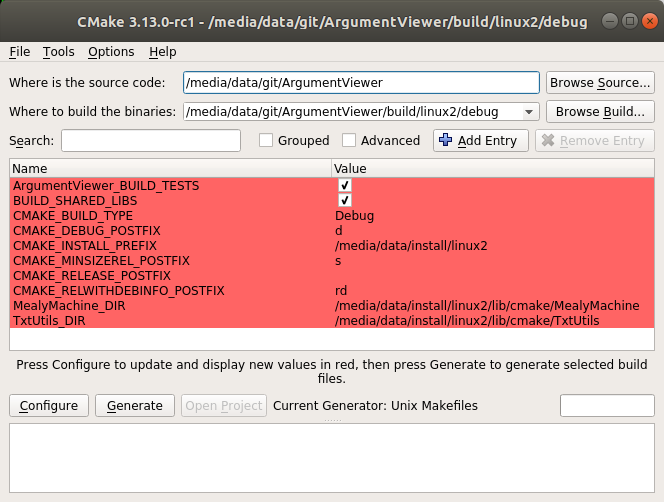
\includegraphics[width=8cm,keepaspectratio]{pics/introduction/cmake-gui}
	\end{figure}
\end{frame}



\setbeamercolor{background canvas}{bg=fitblue}
\begin{frame}
\frametitle{Základní návod}
\begin{center}
\Huge {\color{white}Základní návod}
\end{center}
\end{frame}
\setbeamercolor{background canvas}{bg=white}

\begin{frame}[fragile]
\frametitle{Základní návod}
	\begin{itemize}
	\item Složka obsahující CMakeLists.txt je složka, kterou je možné sestavit
  \item Hierarchie složek
  \item CMake sám o sobě nesestavuje aplikace/knihovny
  \item CMake slouží pro generování makefile / sln souborů
  \item CMake obsahuje aplikace \textbf{cmake cmake-gui ccmake ctest cpack}
  \item \textbf{cmake} - rovnou vygeneruje makefile (parametery můžou ovlivnit generování
  \item \textbf{cmake-gui} / \textbf{ccmake} - uživatelské nastavní parametrů a následné vygenerování makefile
  \item \textbf{ctest} - pro spouštění testů (unit tests, ...)
  \item \textbf{cpack} - pro vytvoření balíčků (*.deb, ...)
	\end{itemize}
\end{frame}

\setbeamercolor{background canvas}{bg=fitblue}
\begin{frame}
\frametitle{Prázdný CMake}
\begin{center}
\Huge {\color{white}Prázdný CMake}
\end{center}
\end{frame}
\setbeamercolor{background canvas}{bg=white}

\begin{frame}[fragile]
\frametitle{Prázdný CMakeLists.txt}
CMakeLists.txt:
\inputminted[frame=lines]{cmake}{../examples/00-EmptyCMake/CMakeLists.txt}
\end{frame}

\setbeamercolor{background canvas}{bg=fitblue}
\begin{frame}
\frametitle{HelloWorld CMake}
\begin{center}
\Huge {\color{white}HelloWorld CMake}
\end{center}
\end{frame}
\setbeamercolor{background canvas}{bg=white}

\begin{frame}[fragile]
\frametitle{HelloWorld CMakeLists.txt}
CMakeLists.txt:
\inputminted[frame=lines]{cmake}{../examples/01-HellowWorld/CMakeLists.txt}
main.cpp:
\inputminted[frame=lines]{c++}{../examples/01-HellowWorld/main.cpp}
\end{frame}

\begin{frame}[fragile]
\frametitle{HelloWorld Sestavení}
CMake umožňuje out-of-source building - vytváření *.o souborů mimo *.cpp soubory.
{\small
\begin{Verbatim}[commandchars=\\\{\}]
$ \textbf{ls}
CMakeLists.txt main.cpp
$ \textbf{mkdir} build
$ \textbf{cd} build
$ \textbf{cmake} ..
$ \textbf{ls}
CMakeCache.txt  \textcolor{blue}{CMakeFiles}  cmake_install.cmake  Makefile
$ \textbf{make}
$ \textbf{ls}
CMakeCache.txt  \textcolor{blue}{CMakeFiles}  cmake_install.cmake  \textcolor{orange}{HelloWorld}  Makefile
\end{Verbatim}
}
\end{frame}

\setbeamercolor{background canvas}{bg=fitblue}
\begin{frame}
\frametitle{Include Directories}
\begin{center}
\Huge {\color{white}Include Directories}
\end{center}
\end{frame}
\setbeamercolor{background canvas}{bg=white}

\begin{frame}[fragile]
\frametitle{IncludeDirectories CMakeLists.txt}
  CMakeLists.txt:
  {\scriptsize \inputminted[frame=lines]{cmake}{../examples/02-IncludeDirectories/CMakeLists.txt}}
  src/main.cpp:
  {\scriptsize \inputminted[frame=lines]{c++}{../examples/02-IncludeDirectories/src/main.cpp}}
  include/header.h:
  {\scriptsize \inputminted[frame=lines]{c++}{../examples/02-IncludeDirectories/include/header.h}}
\end{frame}

\setbeamercolor{background canvas}{bg=fitblue}
\begin{frame}
\frametitle{Compile Definitions}
\begin{center}
\Huge {\color{white}Compile Definitions}
\end{center}
\end{frame}
\setbeamercolor{background canvas}{bg=white}

\begin{frame}[fragile]
\frametitle{Compile Definitions}
  CMakeLists.txt:
  {\scriptsize \inputminted[frame=lines]{cmake}{../examples/03-CompileDefinitions/CMakeLists.txt}}
  src/main.cpp:
  {\scriptsize \inputminted[frame=lines]{c++}{../examples/03-CompileDefinitions/main.cpp}}
\end{frame}

\setbeamercolor{background canvas}{bg=fitblue}
\begin{frame}
\frametitle{Sestavení a instalace knihovny třetí strany}
\begin{center}
\Huge {\color{white}Sestavení a instalace knihovny třetí strany}
\end{center}
\end{frame}
\setbeamercolor{background canvas}{bg=white}

\begin{frame}[fragile]
\frametitle{Sestavení a instalace knihovny třetí strany}
\url{https://github.com/dormon/Vars}
{\scriptsize
\begin{Verbatim}[commandchars=\\\{\}]
$ \textbf{tree}
\textcolor{blue}{.}
|
|-- CMakeLists.txt
|-- main.cpp
|-- \textcolor{blue}{Vars}     \textcolor{gray}{# extern library}
    |-- CMakeLists.txt
    |-- README.md
    |-- \textcolor{blue}{src}
    |   |-- \textcolor{blue}{Vars}
    |       |-- Fwd.h
    |       |-- Resource.cpp
    |       |-- Resource.h
    |       |-- Vars.cpp
    |       |-- Vars.h
    |       |-- VarsImpl.cpp
    |       |-- VarsImpl.h
    |-- \textcolor{blue}{tests}
        |-- catch.hpp
        |-- CMakeLists.txt
        |-- tests.cpp
\end{Verbatim}
}
\end{frame}

\begin{frame}[fragile]
\frametitle{Sestavení a instalace knihovny třetí strany}
{\small
\begin{Verbatim}[commandchars=\\\{\}]
$ \textbf{mkdir} varsBuild
$ \textbf{mkdir} install
$ \textcolor{gray}{# vygenerování makefile}
$ \textcolor{gray}{# -H složka s CMakeLists.txt}
$ \textcolor{gray}{# -B složka pro build}
$ \textcolor{gray}{# -D nastavení parameteru (proměnné)}
$ \textcolor{gray}{# \textcolor{red}{CMAKE_INSTALL_PREFIX} místo pro instalaci knihovny}
$ \textbf{cmake} -H\textcolor{blue}{Vars} -B\textcolor{blue}{varsBuild/} -D\textcolor{red}{CMAKE_INSTALL_PREFIX}=\textcolor{blue}{install/}
$ \textcolor{gray}{# spuštění překladu a instalace}
$ \textcolor{gray}{# --build cesta k build složce}
$ \textcolor{gray}{# --target název cíle, který se bude sestavovat}
$ \textcolor{gray}{# pokud cíl závisí na jiných, nejprve se sestaví ty}
$ \textbf{cmake} --build \textcolor{blue}{varsBuild/} --target install
\end{Verbatim}
}  
\end{frame}

\begin{frame}[fragile]
\frametitle{Sestavení a instalace knihovny třetí strany}
Po instalaci vypadá složka s nainstalovanou knihovnou takto:
\begin{Verbatim}[commandchars=\\\{\}]
$ \textbf{tree} \textcolor{blue}{install/}
|-- \textcolor{blue}{include}
|   |-- \textcolor{blue}{Vars}
|       |-- Fwd.h
|       |-- Resource.h
|       |-- vars_export.h
|       |-- Vars.h
|-- \textcolor{blue}{lib}
    |-- \textcolor{blue}{cmake}
    |   |-- \textcolor{blue}{Vars}
    |       |-- VarsConfig.cmake
    |       |-- VarsConfigVersion.cmake
    |       |-- VarsTargets.cmake
    |       |-- VarsTargets-noconfig.cmake
    |-- libVars.a
\end{Verbatim}
\end{frame}

\setbeamercolor{background canvas}{bg=fitblue}
\begin{frame}
\frametitle{Využití nainstalované knihovny}
\begin{center}
\Huge {\color{white}Využití nainstalované knihovny}
\end{center}
\end{frame}
\setbeamercolor{background canvas}{bg=white}

\begin{frame}[fragile]
\frametitle{Využití nainstalované knihovny}
main.cpp:
{\small \inputminted[frame=lines]{c++}{../examples/04-BuildingAndInstalling/main.cpp}}
CMakeLists.txt:
{\small \inputminted[frame=lines]{cmake}{../examples/04-BuildingAndInstalling/CMakeLists.txt}}
\end{frame}

\begin{frame}[fragile]
\frametitle{Využití nainstalované knihovny}
\begin{Verbatim}[commandchars=\\\{\}]
$ \textbf{ls}
CMakeLists.txt  \textcolor{blue}{install}  main.cpp  \textcolor{blue}{Vars}  \textcolor{blue}{varsBuild}
$ \textbf{mkdir} build
$ \textcolor{gray}{# vygenerování makefile pro aplikaci}
$ \textcolor{gray}{# využívající knihovnu Vars}
$ \textcolor{gray}{# \textcolor{red}{Vars_DIR} je proměnná, která by měla ukazovat na}
$ \textcolor{gray}{# složku, obsahující soubor VarsConfig.cmake}
$ \textbf{cmake} -H\textcolor{blue}{.} -B\textcolor{blue}{build/} -D\textcolor{red}{Vars_DIR}=\textcolor{blue}{install/lib/cmake/Vars}
$ \textcolor{gray}{# sestavení aplikace}
$ \textbf{cmake} --build \textcolor{blue}{build/}
\end{Verbatim}
\end{frame}


\setbeamercolor{background canvas}{bg=fitblue}
\begin{frame}
\frametitle{CMake pro knihovny}
\begin{center}
\Huge {\color{white}CMake pro knihovny}
\end{center}
\end{frame}
\setbeamercolor{background canvas}{bg=white}

\begin{frame}[fragile]
\frametitle{Co požadujeme od CMake pro knihovny?}
	\begin{itemize}
  \item Knihovnu by mělo jít snadno sestavit.
	\item Knihovna by měla jít nainstalovat.
  \item Knihovnu by mělo jít sestavit staticy/dynamicky.
  \item Knihovna by měla propagovat závislosti.
  \item Knihovna by měla vyřešit obtížné závislosti a nepropagovat problémy dál.
  \item Knihovna by měla nastavovat správně cesty k *.lib a *.h
  \item Knihovnu by mělo jít snadno vestavět do většího projektu
  \item Knihovna by neměla předpokládat, že je top most projekt.
  \item Knihovna by měla mít správně verze.
  \item Knihovna by měla mít politiku pro kompatiblitu.
  \item ...
	\end{itemize}
\end{frame}


\begin{frame}[fragile]
\frametitle{Druhy knihoven}
Druhy knihoven:
	\begin{itemize}
	\item dynamické knihovny, sdílené knihovny *.dll *.so
  \item statické knihovny, import knihovny *.lib *.a
  \item header only knihovny *.h
  \item object knihovny *.obj, *.o
  \item plugin/module *.dll *.so
  \item ...
	\end{itemize}
Kde se knihovny hledají, když se pustí aplikace:
	\begin{itemize}
	\item Windows - v místě, kde byla aplikace spuštěna, systémové adresáře, adresáře v proměnné PATH
  \item Linux - zjištění pomocí ldconfig, soubor /etc/ld.so.conf, RPATH, \textbf{ne ve working directory!}
	\end{itemize}
Jak zjistit závislosti knihoven/aplikací:
	\begin{itemize}
	\item Windows - dependency walker
  \item Linux - \textbf{ldd lib.so}, jak zjistit RPATH - \textbf{objdump} -x lib.so $|$ \textbf{grep} -i "runpath"
	\end{itemize}
\end{frame}

\begin{frame}[fragile]
\frametitle{Druhy knihoven II}
Dělení podle druhu kompilace \textcolor{red}{CMAKE\_BUILD\_TYPE}:
	\begin{itemize}
	\item RELEASE knihovny
  \item DEBUG knihovny
  \item RELWITHDEBINFO
  \item MINSIZEREL
	\end{itemize}
Dělení podle toho, jestli ji buildíme my nebo ji od někud dostaneme
  \begin{itemize}
  \item IMPORTED - externí knihovna
  \item SHARED - *.dll+*.lib / *.so
  \item STATIC - *.lib / *.a
  \item OBJECT - *.obj / *.o
  \item INTERFACE - *.h
  \item MODULE - *.dll / *.so
  \item ALIAS - přejmenování
  \end{itemize}
\end{frame}

\setbeamercolor{background canvas}{bg=fitblue}
\begin{frame}
\frametitle{Statická knihovna}
\begin{center}
\Huge {\color{white}Statická knihovna}
\end{center}
\end{frame}
\setbeamercolor{background canvas}{bg=white}

\begin{frame}[fragile]
\frametitle{Statická knihovna}
CMakeLists.txt:
{\scriptsize\inputminted[frame=lines]{cmake}{../examples/05-StaticLibrary/CMakeLists.txt}}
engine.h:
{\scriptsize\inputminted[frame=lines]{c++}{../examples/05-StaticLibrary/engine.h}}
engine.cpp:
{\scriptsize\inputminted[frame=lines]{c++}{../examples/05-StaticLibrary/engine.cpp}}
\end{frame}

\setbeamercolor{background canvas}{bg=fitblue}
\begin{frame}
\frametitle{Sdílená knihovna}
\begin{center}
\Huge {\color{white}Sdílená knihovna}
\end{center}
\end{frame}
\setbeamercolor{background canvas}{bg=white}

\begin{frame}[fragile]
\frametitle{Sdílená knihovna}
CMakeLists.txt:
{\scriptsize\inputminted[frame=lines]{cmake}{../examples/06-SharedLibrary/CMakeLists.txt}}
engine.h:
{\scriptsize\inputminted[frame=lines]{c++}{../examples/06-SharedLibrary/engine.h}}
engine.cpp:
{\scriptsize\inputminted[frame=lines]{c++}{../examples/06-SharedLibrary/engine.cpp}}
\end{frame}

\setbeamercolor{background canvas}{bg=fitblue}
\begin{frame}
\frametitle{Header only knihovna}
\begin{center}
\Huge {\color{white}Header only knihovna}
\end{center}
\end{frame}
\setbeamercolor{background canvas}{bg=white}

\begin{frame}[fragile]
\frametitle{Header only knihovna}
CMakeLists.txt:
{\scriptsize\inputminted[frame=lines]{cmake}{../examples/07-HeaderLibrary/CMakeLists.txt}}
engine.h:
{\scriptsize\inputminted[frame=lines]{c++}{../examples/07-HeaderLibrary/engine.h}}
\end{frame}

\begin{frame}[fragile]
\frametitle{Dobrá knihovna? Část 1.}
{\fontsize{3.5}{3.5}
\begin{minted}[frame=lines]{cmake}
cmake_minimum_required(VERSION 3.13.0)

project(
  MealyMachine
  VERSION 1.0.2
  )

#set these variables to *.cpp, *.c, ..., *.h, *.hpp, ...
set(SOURCES 
  src/${PROJECT_NAME}/MealyMachine.cpp
  )
set(PRIVATE_INCLUDES )
set(PUBLIC_INCLUDES 
  src/${PROJECT_NAME}/Fwd.h
  src/${PROJECT_NAME}/MapTransitionChooser.h
  src/${PROJECT_NAME}/MealyMachine.h
  src/${PROJECT_NAME}/TransitionChooser.h
  src/${PROJECT_NAME}/Exception.h
  )
set(INTERFACE_INCLUDES )

#list of libraries to find
#it should contain list of "lists"
#format:
#set(ExternLibraries
#  A\\ B\\ C\\ D
#  E\\ F\\ G
#  )
#It will be converted into:
#find_package(A B C D)
#find_package(E F G)
#If version is specified, it has to be the second parameter (B)
set(ExternPrivateLibraries )
set(ExternPublicLibraries )
set(ExternInterfaceLibraries )

#set these variables to targets
set(PrivateTargets )
set(PublicTargets )
set(InterfaceTargets )

#set these libraries to variables that are provided by libraries that does not support configs
set(PrivateIncludeVariables )
set(PublicIncludeVariables )
set(InterfaceIncludeVariables )
set(PrivateReleaseLibraryVariables )
set(PublicReleaseLibraryVariables )
set(InterfaceReleaseLibraryVariables )
set(PrivateDebugLibraryVariables )
set(PublicDebugLibraryVariables )
set(InterfaceDebugLibraryVariables )

SET(CMAKE_CXX_STANDARD 14)

set(CMAKE_INCLUDE_CURRENT_DIR ON)
set(CMAKE_INCLUDE_CURRENT_DIR_IN_INTERFACE ON)

option(${PROJECT_NAME}_BUILD_TESTS "toggle building of unit tests")
if(${PROJECT_NAME}_BUILD_TESTS)
  enable_testing()
  add_subdirectory(tests)
  add_test(NAME baseTest COMMAND tests)
endif()
\end{minted}
}
\end{frame}

\begin{frame}[fragile]
\frametitle{Dobrá knihovna? Část 2.}
{\fontsize{2}{2}
\begin{minted}[frame=lines]{cmake}
if("${SOURCES}" STREQUAL "")
  set(HeaderOnly TRUE)
else()
  set(HeaderOnly FALSE)
endif()

#find private dependencies
foreach(lib ${ExternPrivateLibraries})
  list(GET lib 0 libName)
  if(NOT TARGET ${libName}) 
    find_package(${lib})
  endif()
endforeach()

#find public dependencies
foreach(lib ${ExternPublicLibraries})
  list(GET lib 0 libName)
  if(NOT TARGET ${libName}) 
    find_package(${lib})
  endif()
endforeach()


if(NOT ${HeaderOnly})
  option(BUILD_SHARED_LIBS "build this library as shared")
endif()

SET(CMAKE_DEBUG_POSTFIX          "d"  CACHE STRING "add a postfix, usually d on windows"    )
SET(CMAKE_RELEASE_POSTFIX        ""   CACHE STRING "add a postfix, usually empty on windows")
SET(CMAKE_RELWITHDEBINFO_POSTFIX "rd" CACHE STRING "add a postfix, usually empty on windows")
SET(CMAKE_MINSIZEREL_POSTFIX     "s"  CACHE STRING "add a postfix, usually empty on windows")

if(${HeaderOnly})
  add_library(${PROJECT_NAME} INTERFACE)
else()
  add_library(${PROJECT_NAME} ${SOURCES} ${PRIVATE_INCLUDES} ${PUBLIC_INCLUDES} ${INTERFACE_INCLUDES})
endif()

add_library(${PROJECT_NAME}::${PROJECT_NAME} ALIAS ${PROJECT_NAME})

include(GNUInstallDirs)

if(${HeaderOnly})
  target_include_directories(${PROJECT_NAME} INTERFACE $<INSTALL_INTERFACE:${CMAKE_INSTALL_INCLUDEDIR}>)
  target_include_directories(${PROJECT_NAME} INTERFACE $<BUILD_INTERFACE:${CMAKE_CURRENT_SOURCE_DIR}/src>)
else()
  target_include_directories(${PROJECT_NAME} PUBLIC $<INSTALL_INTERFACE:${CMAKE_INSTALL_INCLUDEDIR}>)
  target_include_directories(${PROJECT_NAME} PUBLIC $<BUILD_INTERFACE:${CMAKE_CURRENT_SOURCE_DIR}/src>)
endif()

foreach(inc ${PrivateIncludeVariables})
  target_include_directories(${PROJECT_NAME} PRIVATE ${${inc}})
endforeach()

foreach(inc ${PublicIncludeVariables})
  #this has to be also private because we are exporting this include manually
  target_include_directories(${PROJECT_NAME} PRIVATE ${${inc}})
endforeach()

set(CMAKE_INCLUDE_CURRENT_DIR ON)
set(CMAKE_INCLUDE_CURRENT_DIR_IN_INTERFACE ON)

if(${HeaderOnly})
  target_link_libraries(${PROJECT_NAME} 
    INTERFACE ${InterfaceTargets}
  )
else()
  target_link_libraries(${PROJECT_NAME} 
    PUBLIC    ${PublicTargets} 
    PRIVATE   ${PrivateTargets}
    INTERFACE ${InterfaceTargets}
  )
endif()

if("${CMAKE_BUILD_TYPE}" STREQUAL "RELEASE")
  foreach(lib ${PrivateReleaseLibraryVariables})
    target_link_libraries(${PROJECT_NAME} PRIVATE ${${lib}})
  endforeach()
  foreach(lib ${PublicReleaseLibraryVariables})
    #this has to be also PRIVATE, we are exporting manually...
    target_link_libraries(${PROJECT_NAME} PRIVATE ${${lib}})
  endforeach()
else()
    foreach(lib ${PrivateDebugLibraryVariables})
      target_link_libraries(${PROJECT_NAME} PRIVATE ${${lib}})
    endforeach()
    foreach(lib ${PublicDebugLibraryVariables})
      #this has to be also PRIVATE, we are exporting manually...
      target_link_libraries(${PROJECT_NAME} PRIVATE ${${lib}})
    endforeach()
endif()
\end{minted}
}
\end{frame}

\begin{frame}[fragile]
\frametitle{Dobrá knihovna? Část 3.}
{\fontsize{2}{2}
\begin{minted}[frame=lines]{cmake}
set(PROJECT_NAME_LOWER)
string(TOLOWER ${PROJECT_NAME} PROJECT_NAME_LOWER)

if(NOT ${HeaderOnly})
  include(GenerateExportHeader)
  generate_export_header(${PROJECT_NAME} EXPORT_FILE_NAME ${PROJECT_NAME}/${PROJECT_NAME_LOWER}_export.h)
  set_property(TARGET ${PROJECT_NAME} PROPERTY VERSION ${PROJECT_VERSION})
  set_property(TARGET ${PROJECT_NAME} PROPERTY SOVERSION ${PROJECT_VERSION_MAJOR})
endif()

set_property(TARGET ${PROJECT_NAME} PROPERTY INTERFACE_${PROJECT_NAME}_MAJOR_VERSION ${PROJECT_VERSION_MAJOR})
set_property(TARGET ${PROJECT_NAME} APPEND PROPERTY COMPATIBLE_INTERFACE_STRING ${PROJECT_NAME}_MAJOR_VERSION)

install(TARGETS ${PROJECT_NAME} EXPORT ${PROJECT_NAME}Targets
  LIBRARY  DESTINATION ${CMAKE_INSTALL_LIBDIR}
  ARCHIVE  DESTINATION ${CMAKE_INSTALL_LIBDIR}
  RUNTIME  DESTINATION ${CMAKE_INSTALL_BINDIR}
  INCLUDES DESTINATION ${CMAKE_INSTALL_INCLUDEDIR}
  )

#install header files
if(NOT ${HeaderOnly})
  install(
    FILES       ${CMAKE_CURRENT_BINARY_DIR}/${PROJECT_NAME}/${PROJECT_NAME_LOWER}_export.h
    DESTINATION ${CMAKE_INSTALL_INCLUDEDIR}/${PROJECT_NAME}
    COMPONENT   Devel
    )
endif()

install(
  FILES       ${PUBLIC_INCLUDES} ${INTERFACE_INCLUDES}
  DESTINATION ${CMAKE_INSTALL_INCLUDEDIR}/${PROJECT_NAME}
  COMPONENT   Devel
  )

#create *ConfigVersion.cmake config file
include(CMakePackageConfigHelpers)
set(ConfigDir ${CMAKE_CURRENT_BINARY_DIR}/${PROJECT_NAME})
write_basic_package_version_file(
  ${ConfigDir}/${PROJECT_NAME}ConfigVersion.cmake
  VERSION ${${PROJECT_NAME}_VERSION}
  COMPATIBILITY SameMajorVersion
  )

#create *Targets.cmake config file
export(EXPORT ${PROJECT_NAME}Targets
  FILE      ${ConfigDir}/${PROJECT_NAME}Targets.cmake
  NAMESPACE ${PROJECT_NAME}::
  )

#create content of *Config.cmake config file
string(CONCAT ConfigContent
  "include(CMakeFindDependencyMacro)\n"
  )

foreach(lib ${ExternPublicLibraries} ${ExternInterfaceLibraries})
  list(GET lib 0 libName)
  list(LENGTH lib len)
  if(${len} LESS 2)
    string(CONCAT ConfigContent
      ${ConfigContent}
      "find_dependency(" ${libName} ")\n"
      )
  else()
    list(GET lib 1 libVersion)
    #try to match the version
    string(REGEX MATCH "^[0-9]+(\\.[0-9]+)$" matchedVersion ${libVersion})
    if("${matchedVersion}" STREQUAL "")
      string(CONCAT ConfigContent
        ${ConfigContent}
        "find_dependency(" ${libName} ")\n"
        )
    else()
      string(CONCAT ConfigContent
        ${ConfigContent}
        "find_dependency(" ${libName} " " ${libVersion} ")\n"
        )
    endif()
  endif()
endforeach()


string(CONCAT ConfigContent
  ${ConfigContent}
  "include($" "{CMAKE_CURRENT_LIST_DIR}/${PROJECT_NAME}Targets.cmake)\n"
  )

#create *Config.cmake config file
file(WRITE ${ConfigDir}/${PROJECT_NAME}Config.cmake ${ConfigContent})

#install configs
set(ConfigPackageLocation lib/cmake/${PROJECT_NAME})
install(
  FILES
  ${ConfigDir}/${PROJECT_NAME}Config.cmake
  ${ConfigDir}/${PROJECT_NAME}ConfigVersion.cmake
  DESTINATION ${ConfigPackageLocation}
  COMPONENT   Devel
  )

install(EXPORT ${PROJECT_NAME}Targets
  FILE        ${PROJECT_NAME}Targets.cmake
  NAMESPACE   ${PROJECT_NAME}::
  DESTINATION ${ConfigPackageLocation}
  )
\end{minted}
}
\end{frame}

\begin{frame}[fragile]
\frametitle{Dobrá knihovna? Část 4.}
{\fontsize{2}{2}
\begin{minted}[frame=lines]{cmake}
if((NOT "${PublicIncludeVariables}" STREQUAL "") OR (NOT "${InterfaceIncludeVariables}" STREQUAL ""))

  string(CONCAT FIX
    "\n"
    "# We need to fix libraries that do not provide configs but variables (like GLEW_INCLUDE_DIR GLEW_LIBRARY_RELEASE)\n"
    "# We do it by adding these variables to INTERFACE_INCLUDE_DIRECTORIES and INTERFACE_LINK_LIBRARIES\n"
    "get_target_property(includes " ${PROJECT_NAME} "::" ${PROJECT_NAME} " INTERFACE_INCLUDE_DIRECTORIES)\n"
    "get_target_property(libs " ${PROJECT_NAME} "::" ${PROJECT_NAME} " INTERFACE_LINK_LIBRARIES)\n"
    )
  
  
  foreach(inc ${PublicIncludeVariables})
    string(CONCAT FIX "${FIX}"
      "string(CONCAT includes \\\"\\$" "{includes}\\\" \\\"\;\\$" "{${inc}}\\\")\n"
      )
  endforeach()
  
  foreach(inc ${InterfaceIncludeVariables})
    string(CONCAT FIX "${FIX}"
      "string(CONCAT includes \\\"\\$" "{includes}\\\" \\\"\;\\$" "{${inc}}\\\")\n"
      )
  endforeach()
  
  foreach(lib ${PublicReleaseLibraryVariables})
    string(CONCAT FIX "${FIX}"
      "string(CONCAT libs \\\"\\$" "{libs}\\\" \\\"\\$<\\$<CONFIG:Release>:\;\\$" "{${lib}}>\\\")\n"
      )
  endforeach()
  
  foreach(lib ${InterfaceReleaseLibraryVariables})
    string(CONCAT FIX "${FIX}"
      "string(CONCAT libs \\\"\\$" "{libs}\\\" \\\"\\$<\\$<CONFIG:Release>:\;\\$" "{${lib}}>\\\")\n"
      )
  endforeach()
  
  foreach(lib ${PublicDebugLibraryVariables})
    string(CONCAT FIX "${FIX}"
      "string(CONCAT libs \\\"\\$" "{libs}\\\" \\\"\\$<\\$<CONFIG:Debug>:\;\\$" "{${lib}}>\\\")\n"
      )
  endforeach()
  
  foreach(lib ${InterfaceDebugLibraryVariables})
    string(CONCAT FIX "${FIX}"
      "string(CONCAT libs \\\"\\$" "{libs}\\\" \\\"\\$<\\$<CONFIG:Debug>:\;\\$" "{${lib}}>\\\")\n"
      )
  endforeach()
  
  string(CONCAT FIX "${FIX}"
    "set_target_properties(" ${PROJECT_NAME} "::" ${PROJECT_NAME} " PROPERTIES INTERFACE_INCLUDE_DIRECTORIES \\\"\\$" "{includes}\\\" INTERFACE_LINK_LIBRARIES \\\"\\$" "{libs}\\\")\n"
    )
  
  string(CONCAT installCode 
    "file(APPEND ${CMAKE_INSTALL_PREFIX}/${ConfigPackageLocation}/${PROJECT_NAME}Targets.cmake \"${FIX}\")\n"
    )
  
  install(CODE ${installCode})

endif()
\end{minted}
}
\end{frame}

\begin{frame}[fragile]
\frametitle{Jak řešit závislosti, které mají špatný nebo žádný cmake?}
  Špatné knihovny:
	\begin{itemize}
  \item špatné knihovny poskytují pouze proměnné nikoliv TARGET
  \item špatné knihovny neposkytují instaslaci
  \item špatné knihovny mají špatný install script
  \item špatné knihovny nemají cmake
	\end{itemize}
  Jak řešit?
	\begin{itemize}
  \item Dodat autorům opravený cmake
  \item Napsat / najít Find*.cmake script, který vytvoří target za knihovnu
  \item Distribuovat Find*.cmake script pro závislosti se svojí knihovnou
  \item Vytvořit si ručně IMPORTED TARGET
  \item ...
	\end{itemize}
\end{frame}

\begin{frame}[fragile]
\frametitle{Překopírování DLL do buildu}
{\fontsize{3.7}{3.7}\inputminted[frame=lines]{cmake}{../examples/09-CopyDll/CMakeLists.txt}}
\end{frame}

\begin{frame}[fragile]
\frametitle{Stažení knihovny třetí strany}
{\fontsize{5}{5}\inputminted[frame=lines]{cmake}{../examples/10-Download/CMakeLists.txt}}
\end{frame}




\bluepage{Thank you for your attention! \vspace{10 mm} Questions?}

\end{document}
